\newpage
\section{Auswertung}
\subsection{Kennlinienschar}
Zunächst wird durch die Heizströme $I_{\text{H,}1}$ bis $I_{\text{H,}5}$ der Heizleistung an der Hochvakuumdiode die Ströme $I_1$ bis $I_5$ in Abhängigkeit von der Spannung $U$ abgeschätzt und 
in einer Grafik aufgetragen. Die dazu gehörigen Messwerte werden in der Tabelle \ref{tab:mess1} festgehalten. $I_{\text{H,}1}$ ist $\SI{2.1}{\ampere}$. Die weiteren $I_{\text{H,}x}$ Werte sind im Abstand von 
$\SI{0.1}{\ampere}$ gewählt, sodass $I_{\text{H,}5}$ = $\SI{2.5}{\ampere}$ ist.

\begin{figure}
    \centering
    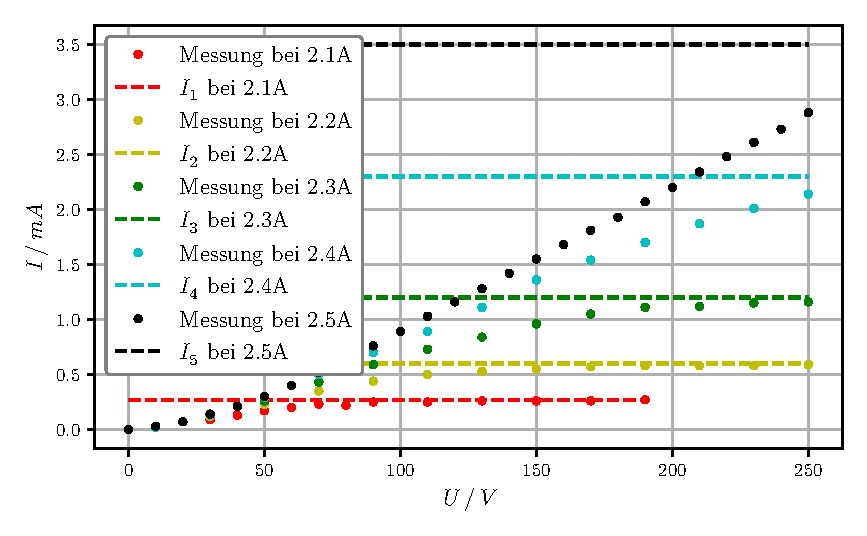
\includegraphics[width=\textwidth]{Daten/kennlinie.pdf}
    \label{fig:kennlinie}
    \caption{Messwerte $I_1$ bis $I_5$ gegen $U$ aufgetragen.}
\end{figure}

Es ist zu erkennen, dass die Ströme eine Sättigung ansteuern. Diese kann lässt sich bei $I_{1}$ bis $I_{3}$ auf ungefähr:

\begin{align*}
    I_\text{S,1} &= \SI{0.27 }{\milli\ampere} \\
    I_\text{S,2} &= \SI{0.6}{\milli\ampere} \\
    I_\text{S,3} &= \SI{1.2}{\milli\ampere}
  \end{align*}

  abschätzen. Bei dem Strom $I_{4}$ kann erahnt werden, dass dieser ungefähr auf einen Wert von $I_\text{S,4}$ = $\SI{2.3}{\milli\ampere}$ zusteuert 
  und bei dem Strom $I_{5}$ lässt sich dieser auf sehr grob auf $I_\text{S,5} = \SI{3.5}{\milli\ampere}$ abschätzen. Diese Abschätzung wird getroffen, da mit all diesen Werten noch später gerechnet wird.

  \begin{table}
  \footnotesize
  \centering
  \caption{Messwerte $I_1$ bis $I_5$}
  \label{tab:mess1}
  \sisetup{table-format=2.1}
  \begin{tabular}{c c c c c c}
  \toprule
  $ U \,/\, \si{\volt} $ & $I_1 \,/\, \si{\milli\ampere}$ & $I_2 \,/\, \si{\milli\ampere}$
  & $I_3 \,/\, \si{\milli\ampere}$ & $I_4 \,/\, \si{\milli\ampere}$ 
  & $I_5 \,/\, \si{\milli\ampere}$ \\
  \midrule 
  0    &  0.00  &  0.00 & 0.00  & 0.00 & 0.00  \\              
  10   &  0.02  &  0.03 & 0.03  & 0.02 & 0.03  \\               
  20   &   -    &   -   &  -    &  -   & 0.07  \\   
  30   &  0.09  &  0.12 & 0.13  & 0.13 & 0.14  \\                  
  40   &  0.13  &   -   &  -    &  -   & 0.21  \\     
  50   &  0.17  &  0.23 & 0.26  & 0.29 & 0.30  \\              
  60   &  0.20  &   -   &  -    &  -   & 0.40  \\     
  70   &  0.23  &  0.35 & 0.43  & 0.50 & 0.52  \\               
  80   &  0.22  &   -   &  -    &  -   & 0.63  \\    
  90   &  0.25  &  0.44 & 0.59  & 0.70 & 0.76  \\              
  100  &   -    &   -   &  -    &  -   & 0.89  \\  
  110  &  0.25  &  0.50 & 0.73  & 0.89 & 1.03  \\               
  120  &   -    &   -   &  -    &  -   & 1.16  \\  
  130  &  0.26  &  0.53 & 0.84  & 1.11 & 1.28  \\             
  140  &   -    &   -   &  -    &  -   & 1.42  \\  
  150  &  0.26  &  0.55 & 0.96  & 1.36 & 1.55  \\               
  160  &   -    &   -   &  -    &  -   & 1.68  \\  
  170  &  0.26  &  0.57 & 1.05  & 1.54 & 1.81  \\               
  180  &   -    &   -   &  -    &  -   & 1.93  \\  
  190  &  0.27  &  0.58 & 1.11  & 1.70 & 2.07  \\               
  200  &   -    &   -   &  -    &  -   & 2.20  \\  
  210  &   -    &  0.58 & 1.12  & 1.87 & 2.34  \\           
  220  &   -    &   -   &  -    &  -   & 2.48  \\  
  230  &   -    &  0.58 & 1.15  & 2.01 & 2.61  \\            
  240  &   -    &   -   &  -    &  -   & 2.73  \\ 
  250  &   -    &  0.59 & 1.16  & 2.14 & 2.88  \\            
  \bottomrule    
  \end{tabular}    
  \end{table}

\subsection{Gültigkeitsbereich des Langmuir-Schottkyschen Raumladungsgesetzes}

Für den maximal mögliche Heizstrom, also $I = 2.5 \si{\ampere}$ wird der Gültigkeitsbereich des Langmuir-Schottkyschen Raumladungsgesetzes untersucht. Dazu wird dieser nochmal in eine 
Grafik eingetragen und es wird ein eine Funktion der Form:
\begin{equation*}
    f = c \cdot V^d    
\end{equation*}

durchgelegt. $c$ und $d$ sind dabei Konstanten. Diese Form ergibt sich durch die Formel (\ref{eqn:anlauf}). Wenn der Gültigkeitsbereich des Langmuir-Schottkyschen Raumladungsgesetzes
auf ungefähr $150 \si{\volt} $ abgeschätzt wird, ergeben sich aus dem Plot die Werte
\begin{align*}
    c &= 0.0010 \pm 0.0001 \\
    d &= 1.458 \pm 0.0197 \; .
\end{align*}

Daraus folgt das der Exponent der Strom-Spannungs-Beziehung $d = 1.458125 \pm 0.019709$ beträgt.

\subsection{Untersuchung des Anlaufstromgebiets}
Nun wird, wie im Kapitel davor, für maximal mögliche Heizleistung das Anlaufstromgebiets untersucht. Dazu wird die Polarisation der Ansaugspannung gedreht und im Intervall von
$0 \si{\volt} $ bis $1 \si{\volt} $ gemessen. Die Messwerte befinden sich in der Tabelle (\ref{tab:mess2}).

Jedoch müssen die gemessenen Werte angepasst werden, da dass Messinstrument, das Nanoamperemeter, einen Widerstand von $R = \SI{1}{\mega\ohm}$
eingebaut hat und durch diesen es zu einem starken Spannungsabfall kommt. Dies kann durch den allgemeinen Zusammenhang $ U = R \cdot I$ kompensiert werden, sodass jeder gemesse Wert 
mit dem Ausgleichstrom verrechnet wird. Mit anderen Worten:

\begin{equation*}
    U_\text{k} = U + I \cdot R \, ,  
\end{equation*}
wobei $U_\text{k}$ den korrigerten Term darstellt. 

\begin{table}
  \centering
  \caption{Messwerte des Diodenstroms im Anlaufstromgebiet}
  \label{tab:mess2}
  \sisetup{table-format=2.1}
  \begin{tabular}{c c c}
  \toprule
  $ U \,/\, \si{\volt} $ & $ U_{\text{k}} \,/\, \si{\volt} $ & $I_5 \,/\, \si{\nano\ampere}$\\
  \midrule 
  0    & 0.0048 &  4.80 \\
  0.1  & 0.1022 &  2.20 \\
  0.2  & 0.20105 &  1.05 \\
  0.3  & 0.3008 &  0.80 \\
  0.4  & 0.40047 &  0.47 \\
  0.5  & 0.50024 &  0.24 \\
  0.6  & 0.6001 &  0.10 \\
  0.7  & 0.70006 &  0.06 \\
  0.8  & 0.80001 &  0.01 \\
  0.9  & 0.900008 &  0.008 \\
  0.97 & 0.97002 &  0.02 \\
  \bottomrule
  \end{tabular}
\end{table}


\begin{figure} [H]
    \centering
    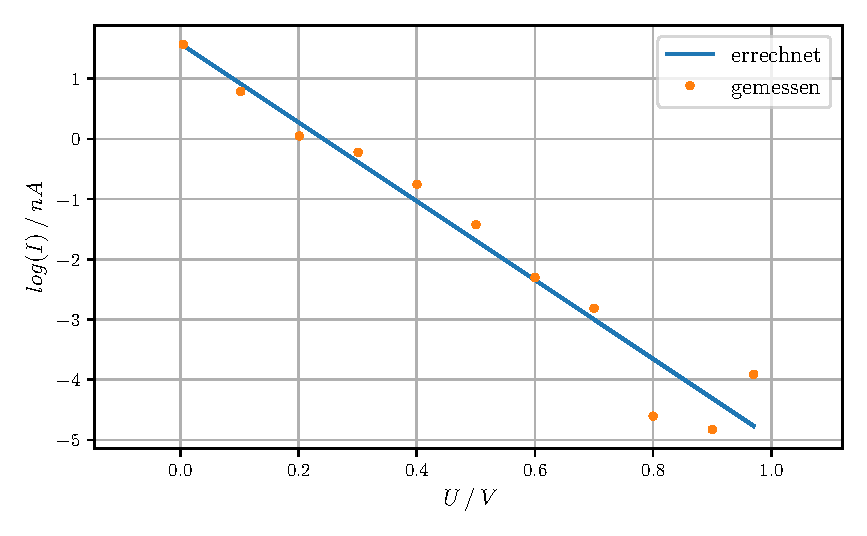
\includegraphics{Daten/gegenfeld.pdf}
    \caption{Kennline der Hochvakkumdiode im Anlaufstromgebiet mit der Heizstromstärke $I = 2.5 \si{\ampere}$}
    \label{fig:3}
\end{figure}


Die korrigerten Werte werden in der Abbildung (\ref{fig:3}) halblogaritmisch gegeneinander aufgetragen. Zusätzlich wird auch hier eine Ausgleichsfunktion, jedoch in diesem Fall in der
Form einer Gerade 
\begin{equation*}
    \text{ln} \left(I \right) = a \cdot U + b
\end{equation*}
durchgelegt. Aus der Rechnung folgt das die Parameter den Wert
\begin{align*}
    a &= -6.5 \pm 0.5\\
    b &= 1.58 \pm 0.28
\end{align*}
haben. Mithilfe der Gleichung \eqref{eqn:anlauf} ergibt sich

\begin{equation*}
      a = - \frac{e}{kT} 
\end{equation*}

und die Temperatur lässt sich durch umstellen 

\begin{equation*}
    T = - \frac{e}{ka} 
\end{equation*}

errechnen zu $ T = 1873.0265 \si{\kelvin}$.

\subsection{Kathodentemperatur bestimmen durch Heizleistungen}
Die Kathodentemperatur lässt sich ebenfalls durch die Leistungsbilanz des Heizstrom-fadens errechnen. Dazu wird der Zusammenhang

\begin{equation}
    \label{eqn:zu}
    \text{N}_\text{zu} = \text{N}_\text{Str} + \text{N}_\text{WL} \,
\end{equation}

genutzt, wobei $\text{N}_\text{zu}$ die zugeführte Leistung ist und $\text{N}_\text{Str}$ und $\text{N}_\text{WL}$ die jeweils abgestrahlte und durch Wärmeleitung an die Apperatur abgegebene Leistung
darstellt.

Mithilfe des Stefan-Boltz-mannschen Gesetzes
\begin{equation*}
    \text{N}_\text{Str} = f \, \sigma \, \eta \, T^4
\end{equation*}

und der Abschätzung von $\text{N}_\text{WL} = 0.95 \si{\watt}$ und $\text{N}_\text{zu} = U_\text{H} \cdot I_\text{H}$, lässt sich die Temperatur berechnen durch

\begin{equation}
    T = \left( \frac{I_\text{H} U_\text{H} - N_\text{WL}}{f \eta \sigma} \right)^{\frac{1}{4}} \, .
    \label{eqn:temp}
\end{equation}

Dabei ist die Stefan-Boltzmannsche Strahlungskonstante $\sigma = \num{5.7e-12}\frac{\text{W}}{\text{cm}^2\text{K}^4}$, die emmitierende Kathodenfläche
$\SI{0.35}{\centi\meter\squared}$ und der Oberflächenemisionsgrad $\eta = \num{0.28}$ gegeben.

Zusätzlich wird die Austrittsarbeit mithilfe der Formel (\ref{eqn:rg}) durch umstellen zu $ e \phi$ berechnen als

\begin{equation}
    e \phi = -k T \: \text{ln} \left( \frac{I_\text{S} h^3}{f 4 \pi e m k^2 T^2} \right) \, .
    \label{eqn:ephi}
\end{equation}

Daraus Folgen die folgenden Werte in der Tabelle (\ref{tab:mess3}).

\begin{table}
    \centering
    \caption{Messwerte der Sättigungsstromstärken, Heizstromstärken und -spannungen, errechneten
            Kathodentemperaturen $T$ und Austrittsarbeiten $e\phi$}
    \label{tab:mess3}
    \sisetup{table-format=2.1}
    \begin{tabular}{c c c c c}
    \toprule
    $I_\text{H} \,/\, \si{\ampere} $ & $U_\text{H} \,/\, \si{\volt}$ & $T \,/\, \si{\kelvin}$
    & $I_\text{S} \,/\, \si{\milli\ampere} $ & $e\phi \,/\, \si{\eV} $\\
    \midrule 
      2,1 & 4,0 & 1954.31 & 0,27& 4.28 \\
      2,2 & 4,1 & 1993.76 & 0,6 & 4.25 \\
      2,3 & 4,8 & 2108.27 & 1,2 & 4.39 \\
      2,4 & 5,0 & 2156.73 & 2,3 & 4.38 \\
      2,5 & 5,5 & 2237.47 & 3,5 & 4.49  \\
    \bottomrule
    \end{tabular}
    \end{table}
  
 Gemittelt beträgt die Austrittsarbeit
  
  \begin{equation*}
      \overline{e\phi} = \SI{4.36 +- 0.04}{\eV} \; .
  \end{equation*}